\documentclass[12pt,letterpaper]{article}


%\usepackage{amsthm}
\usepackage{multirow}
\usepackage{graphicx}
%\usepackage{epsfig}
%\usepackage{subfigure}
\usepackage{amsmath}
\usepackage{indentfirst}
\usepackage{amssymb}
\usepackage{cases}
\usepackage{ dsfont }
\usepackage{mathtools}
\usepackage[figuresright]{rotating}
\usepackage{float}
%\usepackage{subfigure}
\usepackage{caption}
 \usepackage{subcaption}
\usepackage[superscript,biblabel]{cite}

\DeclareMathOperator*{\argmax}{arg\,max}

\usepackage{setspace}
\onehalfspacing


\newtheorem{theorem}{Theorem}
\newtheorem{lemma}{Lemma}
\newtheorem{alg}{Algorithm}
\newtheorem{definition}{Definition}
%{\noindent{\bfseries Proof}}
\newcommand{\Proof}{\noindent{\bfseries Proof}}
%\newcommand{\be}{\begin{equation}}
%\newcommand{\ee}{\end{equation}}
\newtheorem{corollary}{Corollary}
\newtheorem{proposition}{Proposition}
\newtheorem{conjecture}{Conjecture}


\newcommand{\MyTabs}{ \hspace*{15.mm} \= ... \kill }


\usepackage[top=1in, left=1in, right=1in, bottom=1in]{geometry}

\newcommand{\tinyth}{\mbox{{\tiny{th}}}}
\newcommand{\tinyst}{\mbox{{\tiny{st}}}}

\usepackage{sectsty}

\sectionfont{\fontsize{12}{15}\selectfont}

\usepackage{abstract}
\renewcommand{\abstractname}{}    % clear the title
\renewcommand{\absnamepos}{empty} % originally center

\begin{document}
\renewcommand{\refname}{REFERENCES}

\title{XXX}

\author {xxx}%\Large 

\date{}

\maketitle

\begin{abstract}
\noindent\looseness-1
xxx
\end{abstract}

%\begin{keywords}
%Virtual Age, Remote Transmission, Finite Horizon\\
%\end{keywords}
%\centerline{\textsc{acronyms}}
%\begin{tabbing} \MyTabs
%PM\>preventive maintenance \\
%\end{tabbing}
%\centerline{\textsc{notation}}
%\begin{tabbing} \MyTabs
%$L$\> initial system lifetime \\
%\end{tabbing}


%\section*{Introduction}\label{sec:Intro}
%\baselineskip 20pt plus .3pt minus .1pt
\looseness - 1


\section*{Semi-Markov Process (SMP)}\label{sec:Semi Markov Process (SMP)}
\looseness - 1
Semi-Markov processes are a class of stochastic processes which are similar to continuous time markov chains (CTMCs) without the assumption of exponential sojourn time (Kulkarni 2010). The stochastic process of $\{Y(t), t\ge 0\}$ with a countable state space starts in the initial state $Y_0$ at time $t=0$. It goes to the next state ($Y_1$) after remaining there for a sojourn time of $S_1$. In general, this process stays in state $Y_n$ for a sojourn time of $S_{n+1}$ and then jumps to the next state $Y_{n+1}, n\ge 0$. Let $N(t)$ be the number of jumps up to time t. Then the sequence  $\{Y_0, (Y_n, S_n), n\ge 1\}$ is used to define the process $\{Y(t), t\ge 0\}$ by $\{Y(t)=Y_{N(t)}\}$.\\
Therefore, the stochastic process $\{Y_0, (Y_n, S_n), n\ge 1\}$ is called an SMP if it satisfies 
\begin{equation}
P(Y_{n+1}=j, S_{n+1}\le s |Y_n=i, S_n, Y_{n-1}, S_{n-1},..., Y_1, S_1, Y_0)
=P(Y_1=j, S_1\le s |Y_0=i)
\end{equation}

The transition probability from state i to state j at time t is defined as
\begin{equation}
P(Y_{n+1}=j|Y_0, ..., Y_{n-1},Y_{n}=i)=p_{ij}(t)
\end{equation}

and
\begin{equation}
P(S_{n+1}\le s|Y_0, ..., Y_{n-1},Y_{n}=i,Y_{n+1}=j)=H_{ij}^t(x)
\end{equation}

is the distribution function of the sojourn time at state i before transition
to state j at time t.\\
Therefore, the transition distribution at time t will be:
\begin{equation}
P(Y_{n+1}=j, S_{n+1}\le s |Y_n=i)=Q_{ij}^t(x)=p_{ij}(t)H_i^t(x).
\end{equation}

We need to define the following stochastic process:
\begin{equation}

\{N(t); t\geq 0\}= sup\{n\geq 0 : \Sigma_{i=0}^n X_i \leq t\}\\




\end{equation}
and
\begin{equation}
\{N(t); t\geq 0\}
, and \{N(t); t\geq 0\} as:
\end{equation} and 

Consider a two state problem with states: $S=\{1,2\}$ . The changing rate between different states is either constant or duration dependent. The process is the CTMC in the first case and SMP in the second one.\\
We have two separate markov chains of this type. However, the probability of remaining in those states differs in these two markov chains. For instance, in the first chain this probability in states 1 and 2 is $80\%$ and $20\%$ and in the second chain is vice verse. The objective is to minimize the difference of this probability with the average $(50\%)$. 

\begin{figure}[h!]
  \centering
    
      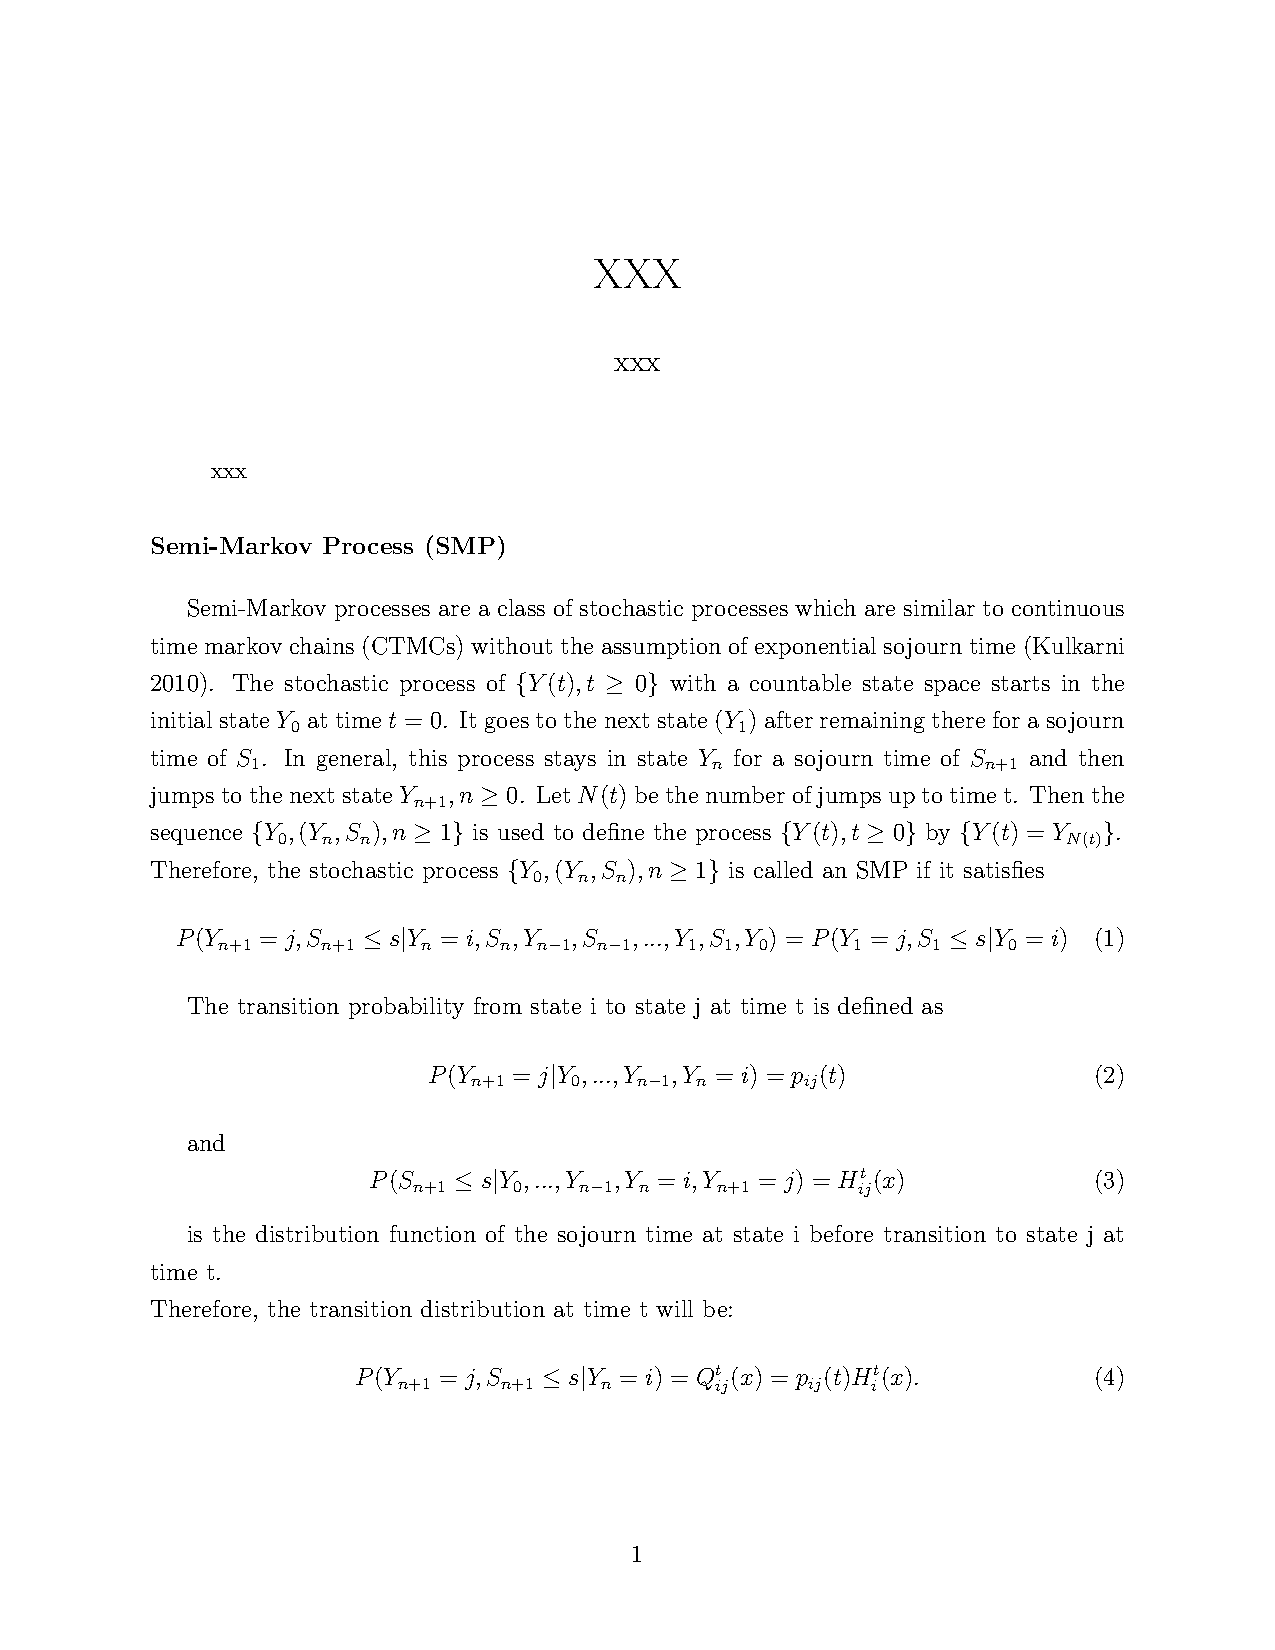
\includegraphics[width=0.5\textwidth]{SMP}
  \caption{Combination of SMP and SMDP}
\end{figure}

Therefore, we want to compute the probabilities of switching between these two states in a time period shorter or equal to $x $. For this goal, we have the following steps:\\
\\
$Y_n=$ State of the system after $n^{th}$ transition.\\
$S_n=$ Sojourn time at transition $n$.\\
$Q_{ij} (x)=$ The conditional probability of going from state $i$ to state $j$ in a time interval of $x$ or shorter.\\
$Q_{ij} (x)=P\{Y_{(n+1)}=j,S_{(n+1)}-S_n\le x|Y_n=i\}$\\
2 states Markov chain:\\

$Q_{12} (x)=\left\{
\begin{array}{c l}      
    1-e^{-\lambda x} &  constant \lambda\rightarrow (CTMC)\\
    1-e^{-\int_{0}^{x} \lambda (y)} & duration-dependent   \lambda(y)\rightarrow     (SMP)
\end{array}\right.$\\


$Q_{21} (x)=\left\{
\begin{array}{c l}      
    1-e^{-\mu x} &  constant \mu\rightarrow (CTMC)\\
    1-e^{-\int_{0}^{x} \mu (y)} & duration-dependent   \mu(y)\rightarrow     (SMP)
\end{array}\right.$\\
\\
The probability of remaining in a state for a specified amount of time x :\\
$Q_{11} (x)=e^{-\int_{0}^{x} \lambda (y)}$\\
$Q_{22} (x)=e^{-\int_{0}^{x} \mu (y)}$
\section*{Semi Markov Decision Process (SMDP)}\label{sec:Semi Markov Decision Process (SMDP)}
\looseness - 1
We can see the problem from the different point of view as a semi markov decision process (SMDP). In this problem, we have two different states as well. However, in each state by choosing an action the transition probability of changing between these different states will be differed. The steps of modeling the problem are as following:\\
 \\
$S=\{S_1,S_2\}$ (States)\\
$A_{(S_1 )}=\{a_{1,1}\} $(Action set of state 1)\\
$A_{(S_2 )}=\{a_{2,1}\} $(Action set of state 1)\\
\\
Transition probabilities for the embedded Markov Decision Process:\\
\\
$ P(S_1 |S_1,a_{1,1} )=0\\
P(S_2 |S_1,a_{1,1 })=1 \\
P(S_2 |S_2,a_{2,1 })=0\\
P(S_1 |S_2,a_{2,1} )=1 $\\
\\
Sojourn time in $S_1$ under $a_{1,1}$ is exponentially distributed: Exp$(\lambda)$\\
Sojourn time in $S_2$ under $a_{2,1}$ is exponentially distributed: Exp$(\mu)$ \\
\\
$Q(t,S_2|S_1,a_{1,1 } )$ : As a consequence of choosing an action$a_{1,1 }\ A_{(S_1 )}$ , the next decision epoch occurs at or before time $t$, and the system state at that decision epoch  equals $ S_2$ with probability of $Q(t,S_2|S_1,a_{1,1 } )$.\\
\\
$F(t|S_1,a_{1,1} )=$ Exp$(\lambda) $ \\
$Q(t,S_2|S_1,a_{1,1 } )=F(t|S_1,a_{1,1} )*P(S_2 |S_1,a_{1,1 })\rightarrow Q(t,S_2|S_1,a_{1,1 } )=$Exp$(\lambda) $ \\
$F(t|S_2,a_{2,1} )=$ Exp$(\mu) $ \\
$Q(t,S_1|S_2,a_{2,1 } )=F(t|S_1,a_{1,1} )*P(S_1 |S_2,a_{2,1 })\rightarrow Q(t,S_1|S_2,a_{2,1 } )=$Exp$(\mu) $ 




\section*{Literature Review}\label{sec:lit_review}
\looseness - 1
\section*{Acknowledgments}
The authors were partially supported by ...
%We also thank the Associate Editor and the anonymous referee for their insightful and constructive comments.



\bibliographystyle{plain}
*\bibliographystyle{unsrt}
*\bibliography{}


%\newpage
%\section{Appendix}\label{app:1}





\end{document}
